%
% report.tex - tex model of graduation work
% Version 0.1
%
% Author: Paulo S. Machado
% Date: June 2010
%
% Release under de GNU Public License v3.0 or greater
% This library is free software; you can redistribute it and/or
% modify it under the terms of the GNU General Public
% License as published by the Free Software Foundation; either
% version 3.0 of the License, or (at your option) any later version.
% 
% This template is distributed in the hope that it will be useful,
% but WITHOUT ANY WARRANTY; without even the implied warranty of
% MERCHANTABILITY or FITNESS FOR A PARTICULAR PURPOSE.  See the GNU
% General Public License for more details.
% 
% You should have received a copy of the GNU Lesser General Public
% License along with this template; if not, write to the Free Software
% Foundation, Inc., 51 Franklin St, Fifth Floor, Boston, MA  02110-1301  USA
%
\documentclass[a4paper,11pt]{article}

% Preamble
%
% preamble.tex - tex model of graduation work
% Version 0.1
%
% Author: Paulo S. Machado
% Date: June 2010
%
% Release under de GNU Public License v3.0 or greater
% This library is free software; you can redistribute it and/or
% modify it under the terms of the GNU General Public
% License as published by the Free Software Foundation; either
% version 3.0 of the License, or (at your option) any later version.
% 
% This template is distributed in the hope that it will be useful,
% but WITHOUT ANY WARRANTY; without even the implied warranty of
% MERCHANTABILITY or FITNESS FOR A PARTICULAR PURPOSE.  See the GNU
% General Public License for more details.
% 
% You should have received a copy of the GNU Lesser General Public
% License along with this template; if not, write to the Free Software
% Foundation, Inc., 51 Franklin St, Fifth Floor, Boston, MA  02110-1301  USA
%
% Language
\usepackage[portuges,brazil]{babel}
\usepackage[top=3cm,bottom=3cm,left=3.0cm,right=3cm]{geometry}
\usepackage[pdftex]{graphicx}
\usepackage{listings}
\usepackage{textcomp}
\usepackage{amssymb}
\usepackage{amsmath}
\usepackage{color}
% Encoding
\usepackage[utf8]{inputenc}

%\usepackage{wrapfig}
%\usepackage{hyperref}

% This will commands into the pdf to create a linked table of contents, as well
%as links for 
% the cross-references such as calls to figure and page numbers 
\usepackage[pagebackref=true]{hyperref}  
\hypersetup{
  pdftitle     = Trabalho de Graduação,
  pdfauthor    = Paulo Silveira Machado,
  colorlinks   = true,
  linkcolor    = black,
  anchorcolor  = red,
  citecolor    = blue,
  filecolor    = red,  
  urlcolor     = red
}



\DeclareGraphicsExtensions{.jpg,.jpeg,.png}
\graphicspath{{../../imagens/}}
% Heading foot
\usepackage{fancyhdr}
\pagestyle{fancy}
\headheight 15pt
\renewcommand{\sectionmark}[1]{\markright{\thesection\ #1}}
\rhead[\fancyplain{}{\bfseries\thepage}] %
    {\fancyplain{}{\bfseries\rightmark}}
\lhead{}
%\lhead[\fancyplain{}{\scshape\leftmark}] %
%    {\fancyplain{}{\bfseries\thepage}}
\cfoot{--~\thepage~--}

\begin{document}

% Title page and table of contents
%
% title.tex - tex model of graduation work
% Version 0.1
%
% Author: Paulo S. Machado
% Date: June 2010
%
% Release under de GNU Public License v3.0 or greater
% This library is free software; you can redistribute it and/or
% modify it under the terms of the GNU General Public
% License as published by the Free Software Foundation; either
% version 3.0 of the License, or (at your option) any later version.
% 
% This template is distributed in the hope that it will be useful,
% but WITHOUT ANY WARRANTY; without even the implied warranty of
% MERCHANTABILITY or FITNESS FOR A PARTICULAR PURPOSE.  See the GNU
% General Public License for more details.
% 
% You should have received a copy of the GNU Lesser General Public
% License along with this template; if not, write to the Free Software
% Foundation, Inc., 51 Franklin St, Fifth Floor, Boston, MA  02110-1301  USA
%
% Title page
\begin{titlepage}
\begin{center}
 
% Header

\includegraphics[width=0.15\textwidth]{figures/unicamp128}\\[1cm]
\textsc{\LARGE Universidade Estadual de Campinas}\\[0.3cm]
\textsc{\LARGE ES952 - Trabalho de Graduação II}\\[3.0cm] 
\textsc{\Large Relatório de Atividades} \\[0.2cm]

  
% Title
\hfill
\textsf{ \LARGE \bfseries Desenvolvimento de um câmbio automático para
bicicletas}

\vfill
% Author and project
\begin{minipage}{0.49\textwidth}
\begin{flushleft} \large
\emph{Autor:}\\
Paulo Silveira Machado \\
RA: 024831
\end{flushleft}
\end{minipage}
\begin{minipage}{0.5\textwidth}
\begin{flushright} \large
\emph{Orientador:} \\
Prof. Dr. Luiz Otávio Saraiva Ferreira\\
Faculdade de Engenharia Mecânica
\end{flushright}
\end{minipage}
 
\vfill
 
% Botton
{\large 2\textordmasculine ~Semestre/2011}
\end{center}
 
\end{titlepage}

% Table of contents
\tableofcontents
\pagebreak

% List of figures
\listoffigures
\pagebreak

% List of tables
\listoftables
\pagebreak


\lstset{frame=single,
    showstringspaces=false,
    extendedchars=true,
    language=C++,
    backgroundcolor=\color[rgb]{0.95,0.95,0.95},
    rulecolor=\color[rgb]{0.3,0.3,0.3},
    basicstyle=\scriptsize\ttfamily,
    commentstyle=\color[rgb]{0.5,0.0,0.0}\rmfamily\itshape,
    keywordstyle=\color[rgb]{0.6,0.0,0.0}\bfseries,
    stringstyle=\color[rgb]{0.6,0.4,0.4},
    identifierstyle=\color[rgb]{0.0,0.0,0.5},
    %numbers = left,
    %numberstyle = \tiny,
    %stepnumber = 2,
    %numberstyle=\color[rgb]{0.0,0.2,0.0},
    basicstyle=\tiny,
}

%%%
%
\section{Resumo}
\label{sec:resumo}
% Breve contexto, função
% Pré requisitos
% Estrutura do documento
% Do que se trata
% Estrutura do texto
A idéia deste projeto surgiu das observações diárias de ciclistas e uso da bicicleta, onde pude perceber
que a maioria das pessoas não sabe utilizar de forma eficiente as marchas de suas bicicletas. Assim como
em uma transmissão automotiva, maus hábitos no seu manejo - esticar marchas, manter a mão apoiada sobre a 
alavanca, entre outros - causam desgaste precoce dos componentes, esforços desnecessários (neste caso para
ciclista) e até risco de segurança. Logo, porque não automatizar este mecanismo de troca de marcha, muito 
mais simples que uma transmissão automotiva?
\\
Este relatório apresenta o desenvolvimento e resultados do trabalho proposto e estudado na primeira 
disciplina de Trabalho de Graduação, onde foram construídas as base teóricas e ferramentais para a construção 
de um protótipo funcional: construção da bancada experimental; desenvolvimento da lógica; e estudo de soluções 
existentes. Ou seja, dados os objetivos do projeto - software de controle, circuito de controle, atuados mecânico 
e a junção destes no protótipo - apresenta-se o caminho percorrido até o objetivo e os resultados alcançados.
\\
O documento foi estruturado de forma a descrever as alternativas, escolhas e desenvolvimento de cada parte funcional
do protótipo final.
% explanação do mecanismo
% partes funcionais
%       microcontrolador
%       cicuito
%       bancada
% inteligência
%       software
% protótipo
% testes
% resultados
% Conclusão
% bibliography
% anexos
%   atuador
%   sensores

\pagebreak
%%%
%
\section{Introdução}
\label{sec:intro}
Problema de engenharia.

\pagebreak
%%%
%
\section{Desenvolvimento das partes}
\label{sec:partes}
O projeto foi dividido em partes, com desenvolvimento em paralelo, para agilizar o processo e para que mudanças no projeto de alguma das partes refletissem imediatamente nas outras. Esta sinergia foi mais forte entre o Circuito de controle (Sec. \ref{sec:arduino}) e o Software de controle (Sec. \ref{sec:software}).

\subsection{Bancada experimental}
\label{sec:bancada}
Criar uma bancada para este projeto sempre foi uma das premissas básicas, tanto que constituia um dos objetivos da primeira parte deste trabalho de graduação. Simular os sinais do sistema via algum tipo de software ou kit não foi considerada como opção, pois nenhuma nuance de um sistema real deveria ser perdida. Logo a solução elaborada no primeiro trabalho foi usar uma bicicleta convencional e transformá-la adequadamente. O resultado é apresentado na Figura \ref{fig:bancada}.
\begin{figure}[!h]
 \begin{center}
  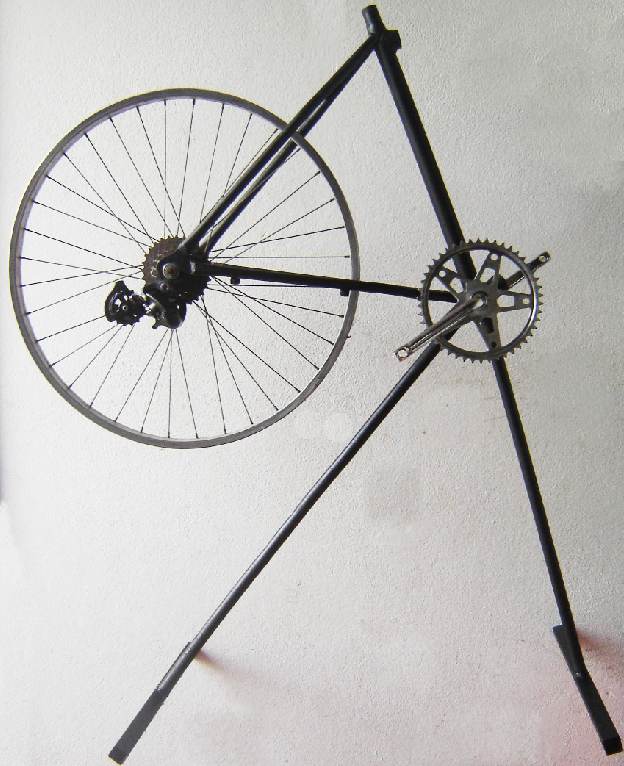
\includegraphics[width=0.50\textwidth]{./figures/bancada_tratada.eps}
 \end{center}
 \caption{Bancada experimental - TG I}
 \label{fig:bancada}
\end{figure}
Ou seja, a bancada é uma meia bicicleta - com a parte traseira, onde estão os elementos da transmissão - onde foram soldados apoios, possibilitando ``pedalar no vazio'' e realizar os testes do projeto, fiel a um cenário real. \\
Os problemas relativos a bancada foram muitos e surgiram no momento prévio aos testes, quando os componentes da transmissão foram montados. As peças disponíveis não foram escolhidas corretamente (corrente curta, coroa dianteira não casou com o corrente), o que causou novos custos e atraso nos testes.

%%%
%
\subsection{Circuito de controle}
\label{sec:arduino}
Arduino\\
botões da constante K \\
Display LCD \\
debounce em hardware e software \\
comunicação serial \\
foto da montagem \\
circuito do pwm \\

%%%
%
\subsection{Software de controle}
\label{sec:software}
No início do projeto houve a intenção de usar técnicas de controle discreto no algoritmo de controle.
Porém a grande dificuldade de modelar o problema físico levou a uma mudança de abordagem, do problema de controle para o problema de automação. Assim, baseado nas entradas e saídas do sistema a lógica apresentada na Figura \ref{fig: fluxograma1} foi elaborada, ainda na primeira parte deste trabalho. 
% Fluxograma
\begin{figure}[!h]
 \begin{center}
  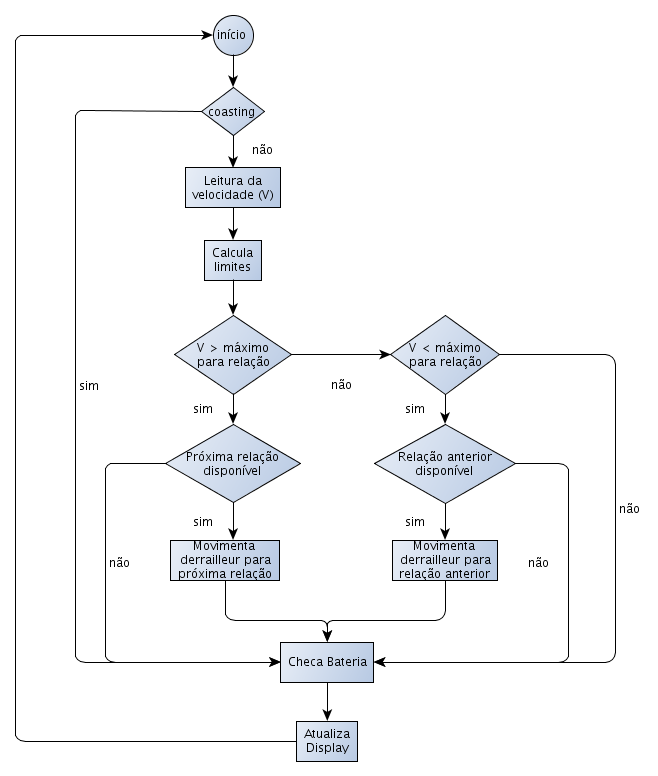
\includegraphics[width=0.80\textwidth]{./figures/fluxograma1}
 \end{center}
 \caption{Lógica de controle inicial}
 \label{fig: fluxograma1}
\end{figure}
Após o início da codificação, algumas 
% evolução da lógica
%TODO fluxograma da máquina de estado

%estrutura do código biblioteca e codigo
 
%%%
%
\subsection{Protótipo}
\label{sec:prototipo}


\pagebreak
%%%
%
\section{Testes e Resultados}
\label{sec:resultados}

\pagebreak
%%%
%
\section{Conclusões}
\label{sec:conclusoes}
% dificuldades
% trabalhos futuros (dinamo e gerenciamento de energia, memoria persistente, ajuste das relações)


\pagebreak
%%%
%
\section{Anexos}
\label{sec:anexos}

%%%
%
\subsection{Elementos sensores}
\label{sensores}
A definição e uso de elementos sensores foi um dos grandes obstáculos deste projeto. Estes deveriam ser usados para a leitura de pulsos a cada revolução da roda e do pedivela, gerando a informação de velocidade básica ao algoritmo de controle. As soluções analisadas foram:
\begin{itemize}
 \item Sensor capacitivo
 \item Sensor indutivo
 \item \textit{Reed switch}
 \item Sensor de efeito HALL
\end{itemize}
Os principais critérios de escolha, que permearam o projeto desde sua concepção, foram simplicidade e custo.
Logo, foi feita a escolha óbvia pelo reed switch, o mais simples e barato entre todos. \\
Porém, os \textit{reed switch} são chaves que geram muito ruído (\textit{bounce}) o sinal gerado precisa de um tratamento para que possa ser aproveitado. Foi considerado realizar o \textit{debounce} do sinal de duas formas: via software; ou via hardware. A primeira foi logo descartada pois as funções do programa responsáveis pelo cálculo de velocidade seriam rotinas de interrupção, ou seja, eles devem ter uma execução muito breve, caso contrário podem afetar a contagem de tempo do sistema. Uma função de \textit{debounce} em software envolve, inerentemente algum \textit{delay}.\\

\begin{figure}[!h]
 \begin{center}
  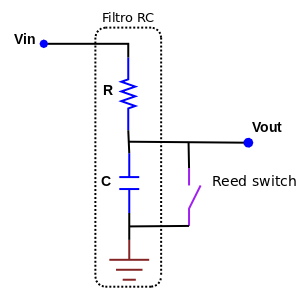
\includegraphics[width=0.20\textwidth]{./figures/lowpass.eps}
 \end{center}
 \caption{Filtro passa-baixa passivo}
 \label{fig: lowpass}
\end{figure}

A única saída foi mesmo implementar o \textit{debounce} em hardware, utilizando um filtro passa-baixa passivo, que usa apenas um resistor e um capacitor, de acordo com o esquema da Figura \ref{fig: lowpass}. O ruído de um \textit{reed switch} comum está na faixa de 1500Hz a 2000Hz\cite{reed}. É possível estimar a frequência máxima ($f_{max}$) de ativação dos \textit{reeds} a partir de um limite de velocidade da roda ($v_{max} = 90 km/h = 25 m/s$):
\begin{center}
$ v = \omega r = 2\pi f r \Rightarrow v_{max} = 2\pi f_{max} r $ 
\end{center}
O diâmetro da roda com pneu foi medido em d =65cm = 0.65m. Portanto, para velocidade máxima de 90 km/h:
\begin{center}
$ f_{max} = \frac{\displaystyle v_{max}}{\displaystyle \pi d} = \frac{\displaystyle 25}{\displaystyle \pi 0.65} = 12.243 Hz $ 
\end{center}
Tomando a frequência de corte ($f_{c}$) dada pela relação,
\begin{center}
 $ f_{c} = \frac{\displaystyle 1}{\displaystyle 2\pi\tau} $, onde $ \tau = RC $
\end{center}
igual a frequência máxima ($f_{max}$), diversas combinações de resistores e capacitores são possíveis. Logo, um pequeno script escrito em pyhton\cite{python} foi usado para ajudar a dimensionar os componentes, de acordo com o que foi adquirido (Sec. \ref{custos}) e o que foi obtido\footnote{Para este trabalho diversos aparelhos - placas mãe, caixas de som, entre outros -  foram canibalizados}.


%%%
%
\subsection{Elemento atuador}
\label{atuador}
Duas perguntas foram elaboradas para ajudar na definição de um atuador: Qual a forma mais simples de atuar sobre um cabo utilizando um motor rotativo? Qual tipo de motor é confiável e fácil de controlar? As repostas são, respectivamente, uma polia e servo motor. \\
O raio da polia foi dimensionado de tal forma que, dado que um servo motor rotaciona 180\textdegree, meia circunferência da polia seja deslocamento suficiente para movimentar o derailleur da menor a maior marcha. Assim, definimos o raio da polia ($r_{polia}$), o número de marchas (n) e o passo (p) como o deslocamento necessário do cabo de comando para a mudança de uma marcha consecutiva, de tal forma que:
\begin{center}
$ \frac{\displaystyle 2\pi r_{polia} }{\displaystyle 2} = (n-1)p $ \\
$ r_{polia} = \frac{\displaystyle (n-1)p}{\displaystyle \pi} $
\end{center}
Para a bancada de testes, n=6 e p=%TODO passo do cabo bancada.
\\O servo motor escolhido foi um Futaba S3004, tal qual o da Figura \ref{fig: servo}. Este possui rolamentos de esferas no eixo de saída, e torque de 4.1kg-cm a 6 volts. O servo drena muita corrente e gera bastante ruído, e portanto teve sua alimentação isolada.

\begin{figure}[!h]
 \begin{center}
  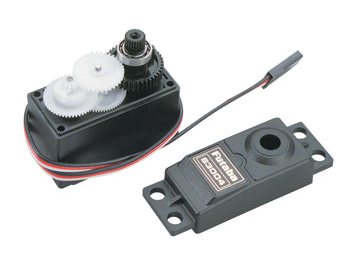
\includegraphics[width=0.50\textwidth]{./figures/S3004.eps}
 \end{center}
 \caption{Servo Futaba S3004}
 \label{fig: servo}
\end{figure}



%%%
%
\subsection{Custos do Projeto}
\label{custos}
Os custos dos materiais utilizados foram relativamente baixos. O reaproveitamento de componentes previamente adquiridos, e principalmente, o baixo custo dos componentes envolvidos possibilitaram minimizar esta soma. A Tabela \ref{tab: custos} a seguir computa os componentes e ferramentas.
{
\newcommand{\mc}[3]{\multicolumn{#1}{#2}{#3}}
\begin{table}[!h]
\begin{center}
\caption{Custos do projeto}
\label{tab: custos}
\begin{tabular}{lc}
\mc{1}{c}{\textbf{Material}} & \textbf{Preço (R\$)}\\\hline
Movimento central & R\$ 12,00\\
Arduino Duemilenove & R\$ 40,00\\
Servo Futaba s3004 & R\$ 12,00\\
Ferro de solda 100W & R\$ 18,00\\
\textit{Reed switch} (5x) & R\$ 3,45\\
Resistores 10k (6x) & R\$ 0,78\\\hline
\textbf{Total} & \textbf{R\$ 86,23}\\\hline
\end{tabular}
\end{center}
\end{table}
}



%%%
%
\subsection{Código integral}
\label{codigo}

\subsubsection{Biblioteca \textit{BikeTransmission}}
\label{code: biblioteca}
Arquivo de cabeçalhos \textit{BikeTransmission.h}:
\begin{lstlisting}
#include </home/paulo/tmp/arduino-0017/build/linux/work/hardware/libraries/Servo/Servo.h>

#ifndef BikeTransmission_h
#define BikeTransmission_h

#endif

/* FrontGear - front sprocket model
 * attributes:
 *
 * methods:
 *  read_cadence_sensor - update period of sprocket cycle
 */
class FrontGear {
public:
    //unsigned long read_cadence_sensor ( int c_reedPin );
};

/* RearWheel - rear wheel model
 * attributes:
 *  diameter - wheel diameter in meters
 * methods:
 *  read_wspeed_sensor - update period of wheel cycle
 *  get_lspeed - calculate and return linear speed
 */
class RearWheel {
public:
    float diameter;
    RearWheel ( float _diameter );
    //unsigned long read_wspeed_sensor ( int w_reedPin );
    int get_lspeed ( long unsigned int T );
};

/* Derailleur - derailleur model
 * attributes:
 *
 * methods:
 *  get_gear - calculate the engaged gear from cycle time ratio
 *  set_gear - decide and move derailleur to appropriate gear
 */
class Derailleur {
public:
    int get_gear ( unsigned long c_t, unsigned long w_t );
    void set_gear ( Servo motor, int gear, long int c_t, long int w_t, float K );
};
\end{lstlisting}
Arquivo de implementação \textit{BikeTransmission.cpp}:
\begin{lstlisting}
#include "BikeTransmission.h"
#include </home/paulo/tmp/arduino-0017/build/linux/work/hardware/libraries/Servo/Servo.h>
#include </home/paulo/tmp/arduino-0017/build/linux/work/hardware/cores/arduino/WProgram.h>

const int GEAR_MAX=6;
const int GEAR_MIN=1;

const int TOTAL_PATH=180;
const int TOTAL_GEARS=6;
const int STEP=TOTAL_PATH/TOTAL_GEARS;

// Time limits (milliseconds)
// 30RPM - 2000ms
const int CADENCE_MIN=3000;
// 90RPM - 667ms
const int CADENCE_MAX=100;

// Offset in the derailleur moviment to engage next gear
const float UP_OFFSET=1.3;
const float DOWN_OFFSET=1.3;

// Debounce time for reed switch.
// This approach limits wheel speed
// to V = pi*D*3.6*1000/T (T stands for
// period in milliseconds
const int DEBOUNCE=70;  // 84 kmph


// Time variables for speed reading:
// c_t - cadence time
// w_t - wheel time
unsigned long c_t1, c_t2, w_t1, w_t2;


/********* Constructors implementation ************/
RearWheel::RearWheel ( float _diameter ) {
    this->diameter = _diameter;
}


/*********** Methods implementation **************/
/*unsigned long FrontGear::read_cadence_sensor ( int c_reedPin ) {
    // TODO actually reads sensor and
    // and return a long integer value
    // in miliseconds. Use ISR
    while ( digitalRead ( c_reedPin ) != HIGH ) ;
    c_t1 = millis();
    delay ( DEBOUNCE );
    while ( digitalRead ( c_reedPin ) != HIGH ) ;
    c_t2 = millis() - DEBOUNCE - c_t1;
    return ( c_t2 );
}


unsigned long RearWheel::read_wspeed_sensor ( int w_reedPin ) {
    // TODO actually reads sensor and
    // and return a long integer value
    // in miliseconds. Use ISR
    while ( digitalRead ( w_reedPin ) != HIGH ) ;
    w_t1 = millis();
    delay ( DEBOUNCE );
    while ( digitalRead ( w_reedPin ) != HIGH ) ;
    w_t2 = millis() - DEBOUNCE - w_t1;
    if ( w_t2 > 5000 ) {
        w_t2 = 0;
    }
    return ( w_t2 );
}*/

// Linear wheel speed:
// V = w*r -> V = 2*pi*f*r
// V = pi*D/T [m/ms]
// V = 3.6*1000*pi*D/T [km/h]
int RearWheel::get_lspeed ( unsigned long T ) {
    // condition to speed less than 1km/h
    if ( ( T > 7350 ) || ( T == 0 ) ) return 0;
    // other condition
    return( int( ( 3.6*3.1416*(this->diameter) )/T*0.001 ));
}

//Return true if param is within tolerance [%] of reference:
boolean closeto(float param, float reference, float tolerance) {
    return ( param >= (reference*(100-tolerance)/100) ) && 
            ( param <= (reference*(100+tolerance)/100) );
}

int Derailleur::get_gear ( unsigned long c_t, unsigned long w_t ) {
    int maxratioindex=5;
    float ratio;
    float validratios[]={ 1.6428571428571428, 1.9166666666666667, 
                          2.2999999999999998, 2.5555555555555554, 2.875, 3.2857142857142856 };
    int gearsforratios[]={ 1,2,3,4,5,6 };
    
    if ( ( c_t != 0 ) || ( c_t > CADENCE_MIN ) ) {
        // These are invariant relations between the bicycle
        // teeth ratios with 5 % tolerance
        // TODO:
        // * Find out the right relations
        // * [beyond TG] configurable ratios
        ratio=c_t/w_t;
        for (int i=0;i<=maxratioindex;i++) {
            if (closeto(ratio,validratios[i],5)) return gearsforratios[i];
        }
        return 0;
    }
    else return 0; // Return code when coasting
}

void Derailleur::set_gear ( Servo motor, int gear, long int c_t, long int w_t, float K ) {
    if ( gear != 0 ) {
        if ( ( c_t < CADENCE_MIN*K ) && ( gear != GEAR_MIN ) ) {
            motor.write (int( STEP* ( gear + 1 ) *UP_OFFSET ));
            //while ( gear == this->get_gear ( c_t, w_t ) ) {
                //Serial.print("Subindo marcha...");
                delay(1000);
            //}
            motor.write ( STEP* ( gear + 1 ) );
        } else if ( ( c_t > CADENCE_MAX*K ) && ( gear != GEAR_MAX ) ) {
            motor.write (int( STEP* ( gear - 1 ) *DOWN_OFFSET ));
            //while ( gear == this->get_gear ( c_t, w_t ) ) {
                //Serial.print("Descendo marcha...");
                delay(1000);
            //}
            motor.write ( STEP* ( gear - 1 ) );
        }
    }
}
\end{lstlisting}

\subsubsection{Programa principal}
\label{code: main}
\begin{lstlisting}
#include <LiquidCrystal.h>
#include <BikeTransmission.h>
#include <Servo.h>


// Objects instatiation
Servo motor;
Derailleur trocador;
LiquidCrystal lcd ( 7, 6, 5, 4, 1, 0 );
RearWheel roda ( 0.65 );
//FrontGear pedivela;

// Constants
const int b0Pin = 11; // K-
const int b1Pin = 12; // K+
const int r0Pin = 3; //Roda
const int r1Pin = 2; //Cadencia
const int pwmPin = 9;
const unsigned int CADENCE_MIN = 2000; // MIN SPEED = MAX TIME

// Variables
unsigned int marcha, wspeed, state=1;
float K=1.00;

// Interrupt used variables
volatile boolean w=false;
volatile boolean c=false;
volatile unsigned long ctime=0;
volatile unsigned long wtime=0;
volatile unsigned long ctimeLog[2];
volatile unsigned long wtimeLog[2];




void setup() {
    //Serial.begin ( 9600 );
    lcd.begin ( 16,2 ); lcd.print( "start up..." );
    delay(2000); lcd.clear(); lcd.print ( "Vel:" );
    lcd.setCursor ( 8,0 ); lcd.print ( "kmph" );
    lcd.setCursor ( 0,1 ); lcd.print ( "Marcha:" );
    lcd.setCursor ( 10,1 ); lcd.print ( "K:" );
    //lcd.setCursor ( 14,0 );
    //lcd.print ( "S" );
    motor.attach ( pwmPin );
    pinMode ( b0Pin, INPUT );
    pinMode ( b1Pin, INPUT );
    pinMode ( r0Pin, INPUT );
    pinMode ( r1Pin, INPUT );
    attachInterrupt ( 1, wheel_monitor, FALLING );
    attachInterrupt ( 0, cadence_monitor, FALLING );
}

void update_lcd() {
    lcd.setCursor ( 4,0 );
    lcd.print("    ");
    lcd.setCursor ( 4,0 );
    lcd.print ( wspeed );
    lcd.setCursor ( 7,1 );
    lcd.print ( marcha );
    lcd.setCursor ( 12,1 );
    lcd.print ( K );
}

void update_serial() {
    Serial.print ( "Velocidade: " ); Serial.print ( wspeed );
    Serial.print ("kmph"); Serial.println ( " " );
    Serial.print ( "Marcha: " ); Serial.print ( marcha ); Serial.println ( " " );
    Serial.print ( "Tempo roda: " ); Serial.print ( wtime );
    Serial.print ( " ms" ); Serial.println ( " " );
    Serial.print ( "Tempo cadencia: " ); Serial.print ( ctime );
    Serial.print ( " ms" ); Serial.println ( " " );
    Serial.print (K); Serial.println ( " " );
    Serial.print (state); Serial.println ( " " );
    Serial.println ( " " );
}

void loop() {
    switch ( state ) {
    case 1:
        update_lcd();
        //update_serial();
        state++;
        break;
    case 2:      
        if (( ctime > CADENCE_MIN ) || ( ctime == 0)) {
            state = 1;
        } else {
            state++;
        }
        break;
    case 3:
        //noInterrupts();
        marcha=trocador.get_gear ( ctime, wtime );
        trocador.set_gear ( motor, marcha, ctime, wtime, K );
        //interrupts();
        state=1;
        break;
    }

    //wspeed = roda.get_lspeed ( wtime );
    wspeed = int( (3.6*3.1416*0.65)/(wtime*0.001) );
    if ( digitalRead ( b1Pin ) == HIGH ) {
        //Serial.print ( "B1" );
        //Serial.println ( " " );
        K=K+0.01;
        if ( K >= 1.5 ) {
            K = 1.5;
        }
    }
    if ( digitalRead ( b0Pin ) == HIGH ) {
        //Serial.print ( "B0" );
        //Serial.println ( " " );
        K=K-0.01;
        if ( K <= 0.5 ) {
            K = 0.5;
        }
    }
    delay ( 500 );

}

void wheel_monitor() {
    if ( w == false ) {
        wtimeLog[0] = millis();
        w=true;
    }
    else {
        wtimeLog[1] = millis();
        wtime = wtimeLog[1] - wtimeLog[0];
        wtimeLog[0] = wtimeLog[1];
    }
}

void cadence_monitor() {
    if ( c == false ) {
        ctimeLog[0] = millis();
        c=true;
    }
    else {
        ctimeLog[1] = millis();
        ctime = ctimeLog[1] - ctimeLog[0];
        ctimeLog[0] = ctimeLog[1];
    }
}
\end{lstlisting}

\subsubsection{\textit{Scripts} auxiliares}
\label{code: helper_scripts}

\lstset{frame=single,
    language=Python,
    basicstyle=\ttfamily\small,
    otherkeywords={1, 2, 3, 4, 5, 6, 7, 8 ,9 , 0, -, =, +, [, ], (, ), \{, \}, :, *, !},
    keywordstyle=\color{blue},
    stringstyle=\color{red},
    showstringspaces=false,
    emph={class, pass, in, for, while, if, is, elif, else, not, and, or,
    def, print, exec, break, continue, return},
    emphstyle=\color{black}\bfseries,
    emph={[2]True, False, None, self},
    emphstyle=[2]\color{key},
    emph={[3]from, import, as},
    emphstyle=[3]\color{blue},
    upquote=true,
    morecomment=[s]{"""}{"""},
    commentstyle=\color{gray}\slshape,
    basicstyle=\tiny,
}

Escritos em python\cite{python} devido a facilidade e rapidez de desenvolvimento nesta linguagem, dois pequenos \textit{scripts} foram usados para: \\
Arquivo ratios.py - Calculo das relações entre marchas, em função do número de dentes das coroas.
\begin{lstlisting}
import os
os.system("clear")

print "Calculate Gear Ratios with Specificied Tolerance:\n"
gears = int(raw_input("Number of gears: "))
tol = float(raw_input("Percentage of tolerance: "))
crown = int(raw_input("Number of teeth in front gear: "))
min = float(crown*(1-tol/100))
max = float(crown*(1+tol/100))
l=[]
l1=[]
l2=[]

for i in range(gears):
    j = int(raw_input("Number of teeth in sprocket %d: " % int(i+1) ) )
    l.append(j)

for i in l:
    l1.append(min/i)
    l2.append(max/i)

if tol != 0:
    print "\nRatios range:"
    for i in range(0,gears):
        print "%sst sprocket:" % int(i+1)
        print "(ratio > %s ) && (ratio < %s)\n" % (l1[i], l2[i])
else:
    print "\nRatios vector:"
    print l1

print "\nDON'T FORGET TO APPLY CHANGES TO C++ CODE!"
\end{lstlisting}

Arquivo capacitance\_n\_resistance.py - calcula ora capacitância, ora resistência necessária para projeto de filtro passa-baixa passivo, a partir de um valor de entrada para a frequência de corte.
\begin{lstlisting}
from decimal import *
import os
os.system("clear")

print "Capacitor and/or Resistor value to reach cutoff frequency"
print "in a simple RC low pass filter. Choose:"

print "1 - Capacitor (resistence input value)"
print "2 - Resistor (capacitance input value)"

i = int(raw_input("Choice [1/2]: "))

if i in [1,2]:
    if i == 1:
        fc = float(raw_input("Cutoff frequency[Hz]: "))
        r = float(raw_input("Resistance [ohm]: "))
        
        print "You need a", Decimal(str(1/(2*3.1416*fc*r))).to_eng_string() ,"F capacitor"
    else:
        fc = float(raw_input("Cutoff frequency[Hz]: "))
        c = float(raw_input("Capacitance [F]: "))
        print "You need a", Decimal(str(1/(2*3.1416*fc*c))).to_eng_string() ,"ohm resistor"
else:
    print "Invalid option", i, ". Exiting...\n"
\end{lstlisting}



\pagebreak
%%%
%
% bibliografia precisa ser explicitamente adicionada ao sumário:
\addcontentsline{toc}{section}{Referências}
\bibliographystyle{plain}
\bibliography{report}

\end{document}